\documentclass[review,3p]{elsarticle}

\usepackage{lineno}       
\modulolinenumbers[5]
\usepackage{subcaption}             % used in subtable
\usepackage{graphicx}
\usepackage{amsmath, amsfonts, amsthm}            % for subequations
\usepackage{mathtools, amssymb}          % for \leqslant
\newcommand{\ddn}[2]{\frac{\mathrm{d}}{\mathrm{d}#1}#2}
\newcommand{\ddt}{\frac{\mathrm{d}}{\mathrm{d}t}}

\usepackage{upgreek}
\usepackage[dvipsnames]{xcolor}
\usepackage{soul}
\usepackage{multirow}

\usepackage{array}
\newcolumntype{C}[1]{>{\centering\let\newline\\\arraybackslash\hspace{0pt}}m{#1}} 
\newcolumntype{L}[1]{>{\raggedright\let\newline\\\arraybackslash\hspace{0pt}}m{#1}} 
\newcolumntype{R}[1]{>{\raggedleft\let\newline\\\arraybackslash\hspace{0pt}}m{#1}} 


\newcommand{\tabitem}{~~\llap{\textbullet}~~}           % for items inside a table
\usepackage{makecell}       % used inside a table
\usepackage{pbox}           % for weak form 3
\usepackage{empheq}
\newcommand*\widefbox[1]{\fbox{\hspace{2em}#1\hspace{2em}}}


\usepackage{colortbl}
\usepackage{esvect}
\usepackage{spreadtab}
\usepackage{numprint}
\usepackage{xstring}
\renewcommand*{\thefootnote}{\fnsymbol{footnote}}
\usepackage[symbol]{footmisc}

\usepackage{siunitx}

\makeatletter       % for rom in deal.ii symbol
\newcommand*{\rom}[1]{\expandafter\@slowromancap\romannumeral #1@}
\makeatother

\usepackage{enumitem}

\usepackage{hyperref}               


\usepackage{cleveref}
\crefformat{section}{\S#2#1#3} 		% see manual of cleveref, section 8.2.1
\crefformat{subsection}{\S#2#1#3}
\crefformat{subsubsection}{\S#2#1#3}

\captionsetup[figure]{labelfont={bf},name={Fig.},labelsep=period}
\captionsetup[table]{labelfont={bf},name={Table},labelsep=space,justification=justified,singlelinecheck=false}      % the last two commands for left-align the caption

\usepackage[labelformat=simple]{subcaption}	        	% order of subfigures with brackets
\renewcommand\thesubfigure{(\alph{subfigure})}
\renewcommand\thesubtable{(\alph{subtable})}

\pdfsuppresswarningpagegroup=1      % eliminate warning 'multiple pdfs with page group included in a single page'

\usepackage[ruled,linesnumbered]{algorithm2e}		% for algorithm
\usepackage{booktabs}       % http://ctan.org/pkg/booktabs


\begin{document}

\begin{frontmatter}

\title{Balancing truncation and round-off errors in practical FEM: one-dimensional analysis}

 \author[1]{Jie Liu\corref{cor1}}
 \ead{j.liu-5@tudelft.nl}
 \author[1]{Matthias Möller}
 \ead{m.moller@tudelft.nl}
 \author[1]{Henk M. Schuttelaars}
 \ead{h.m.schuttelaars@tudelft.nl}
 
 \address[1]{Delft Institute of Applied Mathematics\\ Delft University of Technology\\ Van Mourik Broekmanweg 6, 2628 XE Delft, The Netherlands}
\cortext[cor1]{Corresponding author}

\begin{abstract}
In finite element methods, the solution accuracy cannot be improved indefinitely because of the limited computer precision. We propose an innovative method to find the highest attainable accuracy determined by the round-off error, for the one-dimensional second-order ordinal differential equations. This method uses a priori formula for the error evolution, so that it saves several computations on finer grids. The application of our method to a complex-valued Helmholtz equation in space shows that the highest attainable accuracy can be accurately predicted, while the required CPU time is remarkably saved. 
\end{abstract}


\begin{keyword}
Finite Element Method (FEM), ordinary differential equation, round-off error, highest attainable accuracy, estimation.
\end{keyword}

\end{frontmatter}

\section{Introduction}

Many problems in engineering sciences and industry are modelled mathematically by initial-boundary value problems comprising systems of coupled, nonlinear partial or ordinary differential equations. These problems often consider complex geometries, with initial or boundary conditions that depend on measured data \cite{Kumar2016}. 
In some applications, not only the solution, but also its derivatives are of interest \cite{Kumar2016,carey1982derivative}.
For many problems of practical interest, analytical or semi-analytical solutions are not available, and hence one has to resort to numerical solution methods, such as finite difference, volume and element methods, in which the last will be adopted throughout this paper.

The accuracy of the numerically obtained solution is influenced by many sources of errors \cite{ferziger2012computational}: firstly, errors in the set-up of models, such as the simplification of the realistic domain and governing equations and approximation of initial and boundary conditions; next, truncation errors due to the discretization of the computational domain and use of basis functions for the function spaces defined on it; then, round-off errors due to the adoption of finite-precision computer arithmetics, rather than exact arithmetics; finally, iteration errors resulting from the artificially controlled tolerance of iterative solvers. 

We focus on the error led by the truncation and round-off. One tacitly assumes that the two types of errors are well-balanced. That is, the latter is often ignored based on the argument that it will be `sufficiently small' if just IEEE-754 double-precision floating-point arithmetics are adopted.
However, with the popularity of high-order approximations, the round-off error is likely to play a role with only a small number of degrees of freedom (DoFs) \cite{ling1984numerical,mou2017example,alvarez2012round}. Despite this alarming observation, to the authors’ best knowledge, only very few publications address the impact of accumulated round-off errors on the overall accuracy of the final solution or take them into account explicitly in the error-estimation procedure. The general rule of thumb is still to perform as many $h$-refinements as possible considering the available computer hardware.

The aim of this paper is to systematically analyze the influence of round-off on the error, and to propose a practical approach for obtaining the highest attainable accuracy determined by the round-off error (${E}_{\rm {min}}$).
The scope is restricted to one-dimensional second-order model problems using both the standard finite element method (FEM) and mixed FEM \cite{boffi2013mixed}. We consider the solution and its first and second derivatives, assuming the second derivative exists in the weak sense \cite{necas2011direct}.

The paper is organized as follows. The model problem, finite element formulation and numerical implementation are described in Section \ref{section_model_problem_FEM_formulation_numerical_implementation}. The approach to predicting ${E}_{\rm {min}}$ is discussed in Section \ref{approach_finding_optimal_number_of_DoFs}. The parameters used in the approach are determined in Section \ref{section_error_constants}. An algorithm for realizing the approach and its application to one example are put forward in Section \ref{section_algorithm_application}. The conclusions are drawn in Section \ref{paragraph on conclusion}.

\section{Model problem, finite element formulation and numerical implementation}	\label{section_model_problem_FEM_formulation_numerical_implementation}

\subsection{Model problem}

Consider the following one-dimensional second-order differential equation:
\begin{equation}
  -\left(d(x) u_x \right)_x + r(x)u(x) = f(x),\qquad x \in I = [0,1],	\label{1d_second_order_differential_equation}
\end{equation}
with $u$ denoting the unknown variable, which can either be real or complex, $f(x) \in L^2 (I)$ a prescribed right-hand side, and $d(x)$ and $r(x)$ continuous coefficient functions.
By choosing $d(x)=1$ and $r(x)=0$, Eq. (\ref{1d_second_order_differential_equation}) reduces to the Poisson equation; for $d(x)>0$ and not constant, the diffusion equation is found when $r(x)=0$, and the Helmholtz equation \citep{haberman2012applied} is found when $r(x) \neq 0$. 
The boundary conditions are $u(x)=g(x)$ on $\Gamma_D$ and $d(x)u_x=h(x)$ on $\Gamma_N$, where $\Gamma_D$ and $\Gamma_N$ are the boundaries where Dirichlet and Neumann boundary conditions are imposed, respectively.

\subsection{Finite element formulation} 	\label{FE formulation}

For convenience, we introduce two inner products \citep{lipschutz2009linear}:
 \begin{subequations}
  \begin{align}
	\langle f_1, \,f_2 \rangle &= \int _I f_1(x) f_2(x) \, dx,	\\
   \langle f_1, \,f_2 \rangle _{\Gamma} &= f_1(x_0) f_2(x_0).
  \end{align}
 \end{subequations}
where $f_1(x)$ and $f_2(x)$ are continuous functions defined on $I$, and $x_0$ the coordinate of the boundary $\Gamma$.

\subsubsection{The standard FEM}

The weak form of Eq. (\ref{1d_second_order_differential_equation}) is derived in \ref{derivation_weak_form_SM}. Imposing the Dirichlet boundary conditions strongly, the weak form reads:
\begin{equation}
\centering
\boxed{ 
\begin{aligned}
&\text{Weak~form}~ 1 ~~~~~~~~~\\
&\text{Find $u \in H _D^1 (I)$ such that:} \\
&\langle {\eta} _{ x }, \, du _{ x } \rangle + \langle\eta, \, ru\rangle = \langle\eta, \, f \rangle + \langle\eta, \, hn\rangle_{\Gamma _N} \qquad \forall \eta \in H _{D0}^1 (I),\\
&\text{with} \\
&~~~~~~~~~~~~~H_{D} ^1 (I) = \{t \; | \; t \in H^1 (I), \; t = g \text{ on } \Gamma _D \},  \\
&~~~~~~~~~~~~H_{D0} ^1 (I) = \{t \; | \; t \in H^1 (I), \; t = 0 \text{ on } \Gamma _D\},\\
&\text{where } {n} \text{ is 1 at $x=1$, and $-1$ at $x=0$.}
\end{aligned}		\label{1D_general_SM_weak_form_Diri_strong} 
}
\end{equation}
Imposing the Dirichlet boundary conditions in the weak sense \cite{freund1995weakly}, the weak form reads:
\begin{equation}
\centering
\boxed{
\begin{aligned}
&\text{Weak~form}~ 2 ~~~~~~~~~\\
&\text{Find } u \in H ^1 (I) \text{ such that:}\\
& \langle { \eta} _{ x }, \, du_x \rangle + \langle \eta, \, ru \rangle - \langle \eta, \, du_x n \rangle_{\Gamma _D} + \langle \eta _x, \, u n \rangle_{\Gamma _D} - \langle \eta, \, \rho u n \rangle_{\Gamma _D} \\ 
&= \langle \eta, \, f \rangle + \langle \eta, \, h n \rangle_{\Gamma _N} + \langle \eta _x, \, g n \rangle_{\Gamma _D} - \langle \eta, \, \rho g n \rangle_{\Gamma _D} \qquad \forall \eta \in H ^1 (I), \\
&\text{where } \rho \text{ is a } \text{{positive}} \text{ value that serves as the penalty parameter}.
\end{aligned}	\label{1D_general_SM_weak_form_Diri_weak}
}
\end{equation}

\noindent Note that, the terms in the right-hand sides of Eqs. (\ref{1D_general_SM_weak_form_Diri_strong})--(\ref{1D_general_SM_weak_form_Diri_weak}) consist of information of Neumann boundary conditions which vanish if they are not prescribed. We approximate $u$ by a linear combination of a finite number of basis functions:
\begin{equation}
 u \approx u_h ^{(p)} = \sum _ {i=1} ^{m} u _{i} \varphi _{i}^{(p)}. \label{General_SM_u_approx}%
\end{equation}
Here, $m$ is the number of DoFs, $\varphi _{i}^{(p)}$ are $C^0$-continuous Lagrange basis functions supported by Gauss-Lobatto points, $u_i$ are the values of $u_h^{(p)}$ at the DoFs, and $p$ is the element degree. The resulting linear system of equations reads
\begin{equation}
 A {U} = F,				\label{matrix equation std FEM}
\end{equation}
where $A$ is the stiffness matrix, $F$ the right-hand side and $U$ the discretized $u$.

\subsubsection{The mixed FEM}
Derived in \ref{derivation_weak_form_MM}, the weak form of Eq. (\ref{1d_second_order_differential_equation}) using the mixed FEM is given by:
\begin{subequations}
\begin{empheq}[box=\fbox]{align}
&\text{Weak~form}~ 3 ~~~~~~~~~\notag\\
&\text{Find $v \in H_{N}^1 (I)$ and $u \in L ^2 (I)$ such that:}	\notag\\
& ~~~~~~~\;\langle w, \, d^{-1}v \rangle - \langle w_x, \,  u \rangle = -\langle w, \, g n \rangle_{\Gamma_D} \qquad \forall w \in H_{N0}^1 (I), \label{1D_General_MM_weak_1}\\ 
& ~~~~~~~~~- \langle q, \, v_x \rangle - \langle q, \, ru \rangle = -\langle q, \, f \rangle \qquad \forall q \in L ^2 (I), \label{1D_General_MM_weak_2}	\\
&    \text{with}\notag\\
& ~~~~~~~~~~~~~~~ H_{N} ^1 (I) = \{t \; | \; t \in H^1 (I), \; t = -h \text{ on } \Gamma _N \},  \notag\\
& ~~~~~~~~~~~~~\, H_{N0} ^1 (I) = \{t \; | \; t \in H^1 (I), \; t = 0 \text{ on } \Gamma _N\}.	\notag 
\end{empheq}
\label{1D_General_MM_weak_2in1}%
\end{subequations}
We approximate $v$ and $u$ by:
\begin{subequations}
 \begin{align}
 v \approx v _h^{(p)} &= \sum _ {i=1} ^{n} v _{i} \varphi _{i}^{(p)},     \label{General_MM_var_approx1}  \\[3ex]
 u \approx u _h^{(p-1)} &= \sum\limits _ {j=1} ^{p} u _{tj} \psi _{j}^{(p-1)}, \text{ in cell }t,  \label{General_MM_var_approx2}
\end{align}	\label{General_MM_var_approx}%
\end{subequations}
where $n$ is the number of DoFs for $v_h^{(p)}$, $\varphi _{i}^{(p)}$ are of the same type of basis functions used in Eq. (\ref{General_SM_u_approx}), and $v_i$ are the values of $v_h$ at the DoFs; $\psi _{j}^{(p-1)}$ are discontinuous Lagrange basis functions and $u_{tj}$ are the values of $u_h^{(p-1)}$ at the DoFs. 
The resulting coupled linear system of equations that has to be solved reads:
\begin{equation}
 \left[ \begin{array}{cc} M & B  \\ B^\top & 0 \end{array}\right] \left[ \begin{array}{cc} {V} \\ {U} \end{array}\right] =\left[ \begin{array}{cc} G \\ H \end{array}\right], \label{matrix equation mix FEM}
\end{equation}
where the mass matrix $M$, discrete gradient operator $B$, and its transpose, the discrete divergence operator $B^\top$, comprise the left-hand side; $G$ and $H$ are the components of the right-hand side; $V$ and $U$ are the discretized $v$ and $u$.

For the sake of readability, we will drop the superscript ($p$) or ($p$-1) whenever the approximation order is clear
from the context.

\subsection{Numerical implementation}

\subsubsection{Solution technique}
All results are computed in IEEE-754 double precision \cite{zuras2008ieee} using the deal.\rom{2} finite element code \cite{alzetta2018deal}. 
1) The computational mesh is obtained by globally refining a single element that covers the interval $I$; 
2) the Dirichlet boundary conditions are imposed strongly;
3) sufficiently accurate Gaussian quadrature formulas are used to compute the occurring integrals;
4) the UMFPACK solver \cite{davis2004algorithm} is used to solve the system of equations;
5) the derivatives of the numerical solution are computed in the classical finite element manner, e.g. $u_{h,x}=\sum\limits _{i=1}^m u_i\varphi_{i,x}$ yields an approximation to $u_x$ using standard FEM. 

\subsubsection{Error estimation}

For the numerical results $var_h$ of the variable $var$, the error measured in the $L_2$ norm is used. It is defined as
\begin{subequations}	\label{formula_abs_error}
\begin{align}		\label{formula_abs_error_analytical}
 E_{h} &= {\|var_{h}- {var}_{\rm exc}\|_{2}}
\end{align}
when the exact approximation ${var}_{\rm exc}$ is available, or \cite{Runborg2012VerifyingNC}
\begin{align}		\label{formula_abs_error_numerical}
 {\widetilde {E_{h}}} &= {\|var_{h}- {var}_{h/2}\|_{2}}
\end{align}
otherwise,
\end{subequations}
where $var_{h/2}$ is the numerical solution computed on a mesh of grid size $h/2$. 
Furthermore, we compute the order of convergence from either
\begin{subequations}	\label{formula_order_of_convergence}
\begin{align}		\label{formula_order_of_convergence_analytical}
Q &= \log _2 \left( \frac{E_{h}}{E_{h/2}} \right),
\end{align}
or 
\begin{align}		\label{formula_order_of_convergence_numerical}
\widetilde{Q} &= \log _2 \left( \frac{\widetilde {E_{h}}}{\widetilde {E_{h/2}}} \right),
\end{align}
\end{subequations}
for which the theoretical value is one order higher than the approximation order \cite{gockenbach2006understanding}.


\section{Approach to finding the highest attainable accuracy}                 \label{approach_finding_optimal_number_of_DoFs}

\subsection{Error Evolution}

The conceptual sketch of $E_h$ against the number of DoFs ($N_h$) in the log-log axes can be found in Fig.~\ref{error_evolution_one_p} \cite{butcher2016numerical}.
When $N_h$ is relatively small, $E_h$ may not decrease at the aforementioned theoretical order of convergence, but it basically does when $N_h$ is relatively large.  The transition from the first phase, denoted by the black circles, to the second phase, denoted by the green circles, is usually fast \cite{butcher2016numerical}. $E_h$ in these two phases is controlled by the truncation error, denoted by $E_{\rm T}$, and it can be represented by 
\begin{equation}
 E_{h} \approx E_{\rm T} = \alpha_{\rm T}{N_{h}}^{-\beta_{\rm T}},		\label{formula_truncation_error}
\end{equation}
in the latter phase, where $\alpha_{\rm T}$ is the offset and $\beta_{\rm T}$ is the slope of the line approximating $E_h$. $\beta_{\rm T}$ is also the theoretical order of convergence.

When $N_h$ is even larger, since the domination of the round-off error, denoted by $E_{\rm R}$, $E_h$ increases, see the orange circles. The slope of the line approximating $E_h$, denoted by $\beta_{\rm R}$, tends to be fixed \cite{Babuska2018Roundoff,WalterFrei}, and its value, together with that of the offset, denoted by $\alpha_{\rm R}$, is fixed in Section \ref{section_error_constants}. Thereby, $E_h$ reading
\begin{equation}
 E_{h} \approx E_{\rm R} = \alpha_{\rm R}{N_{h}}^{\beta_{\rm R}},		\label{formula_round_off_error}
\end{equation}
can be predetermined in this phase.


 \begin{figure}[!ht]
 \centering
     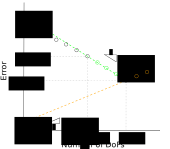
\includegraphics[width=0.5\linewidth]{../2_figure/1_error_evolution_one_p/sketch_error_one_p.pdf}
     \caption{Conceptual sketch of the error evolution against the number of $\text{DoFs}$.}
     \label{error_evolution_one_p}
 \end{figure}

\subsection{Implementation process}           \label{section_strategy}

At the beginning of the second phase, where $E_h$ and $N_h$ are ${E_{\rm c}}$ and ${N_{\rm c}}$, respectively, the offset $\alpha_{\rm T}$ can be inverted by using
\begin{equation}
 \alpha_{\rm T} = {E_{\rm c}}/{N_{\rm c}}^{- \beta_{\rm T}}.		\label{formula_offset_truncation_error}
\end{equation}
Thereafter, both the evolution of $E_{\rm T}$ and $E_{\rm R}$ are known. Obviously, $N_{\rm opt}$ occurs when $E_{\rm T}+E_{\rm R}$ is the smallest. By solving
\begin{equation}
    \frac{d(E_{\rm T}+E_{\rm R})}{dN}=0,    \label{derivative_condition_N_opt}
\end{equation}
we can predict the optimal number of DoFs
\begin{subequations}
\begin{align}
 N_{\rm opt} = \left( \frac{\alpha_{\rm T} \beta_{\rm T}}{\alpha _{\rm R} \beta_{\rm R}} \right)^{\frac{1}{\beta_{\rm T} + \beta_{\rm R}}},
\end{align}
and hence, the highest attainable accuracy
\begin{align}
 E_{\rm min} = \alpha_{\rm T} {N_{\rm opt}}^{- {\beta _{\rm T}}}+\alpha_{\rm R} {N_{\rm opt}}^{{\beta _{\rm R}}}.
\end{align}
\end{subequations}

\section{Determination of the error constants in Fig.~\ref{error_evolution_one_p}}  	\label{section_error_constants}

We determine $\alpha_{\rm R}$ and $\beta_{\rm R}$ for the real-valued problems with only Dirichlet boundary conditions, and then validate them for problems of complex numbers and Neumann boundary conditions.

\subsection{Real-valued problems with only Dirichlet boundary conditions}
\subsubsection{One element degree}

For $p$=2 and $p$=4 for the standard FEM and mixed FEM, respectively, we consider the following equations.
The Poisson equations with $u(x)$ in Table \ref{scaling_cases_Poisson}, for which the distribution of $\|u\|_2$ and $\|f\|_2$ is shown in Fig.~\ref{l2_norm_u_f} for Cases 1--4; the diffusion equations with $d(x)$ in Table~\ref{d_diffusion_equations} and the Helmholtz equations with $d(x)$=1 and $r(x)$ taken from the above constant $d(x)$, for which $u$ is that of Case 1 with $c$=1 in Table \ref{scaling_cases_Poisson}.

\begin{table}[!ht]
\centering
\caption [w]{Settings of the Poisson equations with various $\|u\|_2$ and $\|f\|_2$.} 
\label{scaling_cases_Poisson}
 \begin{tabular}{c l l c} \hline      
Case & $f(x,c)$ & $u(x,c)$ & $c$ \\ \hline
1 & $\makecell{-e^{-{c}{(x-1/2)^2}} \cdot \\ \left({4{c}^2(x-1/2)^2 -2c} \right)}$ & $e^{-{c}{{(x-1/2)^2}}}$ & {1e-4, 1e-2, 1e0, 1e2, 1e4} \\ \hline
2 & $\sin (2 \pi cx)$ & ${(2 \pi c)}^{-2} \sin (2 \pi cx)$ & \multirow{2}{*}{1e-2, 1e-1, 1e0, 1e1, 1e2} \\ \cline{1-3}
3 & $(2 \pi c) \sin (2 \pi c x)$ & ${(2 \pi c)}^{-1} \sin (2 \pi cx)$ &  \\ \hline
4 & $\sin (2 \pi c x) +1$ & ${(2 \pi c)}^{-2}\sin (2 \pi c x)-\frac{x^2}{2}$ & \multirow{2}{*}{1e-4, 1e-2, 1e0, 1e2, 1e4} \\ \cline{1-3}
5 & $0$ & ${c}^{-1} x$ &  \\ \hline
\end{tabular}
\end{table}

\begin{figure}[!ht]
\centering
    \includegraphics[width=0.42\linewidth]{../2_figure/2_l2_norm_u_f/l2_norm_u_f.pdf}
    \caption{Distribution of $\|u\|_2$ and $\|f\|_2$ for the Poisson equations in Table~\ref{scaling_cases_Poisson}.}
    \label{l2_norm_u_f}
\end{figure}


\begin{table}[!ht]
\centering
\caption [w]{Various $d(x)$ for the diffusion equations.} 
\label{d_diffusion_equations}
 \begin{tabular}{c c c c c c} \hline
Order &$d(x)$ & $\|d\|_2$ & Order &$d(x)$ & $\|d\|_2$ \\ \hline
1 & 0.01 & 0.01 & 7 & $1+\sin(10x)$ & 1.14 \\ \hline
2 & 0.1 & 0.1 & 8 & $1+\sin(100x)$ & 1.06 \\ \hline
3 & 1 & 1 & 9 & $1+x$ & 1.5 \\ \hline
4 & 10 & 10 & 10 & $1+10x$ & 6.7 \\ \hline
5 & 100 & 100 & 11& $1+100x$ & 58.6 \\ \hline
6 & $1+\sin(x)$ & 1.23 & & &  \\ \hline
\end{tabular}
\end{table}

\newpage
For all the three types of equations except for Case 5 in Table \ref{scaling_cases_Poisson}, for which only the round-off error exists, the error basically evolves according to that shown in Fig.~\ref{error_evolution_one_p}. To summarize, $\beta_{\rm R}$ is 2 using the standard FEM and 1 using the mixed FEM. $\alpha_{\rm R}$ is shown in Figs.~\ref{py_offset_summary_Pois} -- \ref{py_offset_summary_Helm}, respectively. In Fig.~\ref{py_offset_summary_Pois_sm}, the ratio is 2e-17, 5e-17 and 5e-16 for $u$, $u_x$ and $u_{xx}$, respectively. In Fig.~\ref{py_offset_summary_Pois_mm}, of which the $x$ axis is $\|u\|_2$ for $u$ and $v$, and $\|v\|_2$ for $v_x$, the ratio is 1e-18, 1e-16 and 5e-16 for $u$, $v$ and $v_x$, respectively. In Fig.~\ref{py_offset_summary_diff_mm}, the ratio is 2e-16 and 5e-16 for $v$ and $v_x$, respectively. Therefore, $\alpha_{\rm R}$ can be expressed as the product of a constant, for which a larger value is adopted, and an unknown that are shown in Table~\ref{relation_alpha_R_l2_norm}.

\begin{figure}[!ht]
	\centering
    \begin{subfigure}{6.0cm}
        \includegraphics[width=1.0\linewidth]{../2_figure/4_offset_summary/py_offset_summary_Pois_sm.pdf}
        \caption{The standard FEM}
        \label{py_offset_summary_Pois_sm}
    \end{subfigure}
    \hspace{-0.2cm}
    \begin{subfigure}{6.0cm}
        \includegraphics[width=1.0\linewidth]{../2_figure/4_offset_summary/py_offset_summary_Pois_mm.pdf}
        \caption{The mixed FEM}
        \label{py_offset_summary_Pois_mm}
    \end{subfigure}
\caption{$\alpha_{\rm R}$ for the influence of $u(x)$.}
\label{py_offset_summary_Pois}
\end{figure}

\begin{figure}[!ht]
	\centering
    \begin{subfigure}{6.0cm}
        \includegraphics[width=1.0\linewidth]{../2_figure/4_offset_summary/py_offset_summary_diff_sm.pdf}
        \caption{The standard FEM}
        \label{py_offset_summary_diff_sm}
    \end{subfigure}
    \hspace{-0.2cm}
    \begin{subfigure}{6.0cm}
        \includegraphics[width=1.0\linewidth]{../2_figure/4_offset_summary/py_offset_summary_diff_mm.pdf}
        \caption{The mixed FEM}
        \label{py_offset_summary_diff_mm}
    \end{subfigure}
\caption{$\alpha_{\rm R}$ for the influence of $d(x)$.}
\label{py_offset_summary_diff}
\end{figure}

\begin{figure}[!ht]
	\centering
    \begin{subfigure}{6.0cm}
        \includegraphics[width=1.0\linewidth]{../2_figure/4_offset_summary/py_offset_summary_Helm_sm.pdf}
        \caption{The standard FEM}
        \label{py_offset_summary_Helm_sm}
    \end{subfigure}
    \hspace{-0.2cm}
    \begin{subfigure}{6.0cm}
        \includegraphics[width=1.0\linewidth]{../2_figure/4_offset_summary/py_offset_summary_Helm_mm.pdf}
        \caption{The mixed FEM}
        \label{py_offset_summary_Helm_mm}
    \end{subfigure}
\caption{$\alpha_{\rm R}$ for the influence of $r(x)$.}
\label{py_offset_summary_Helm}
\end{figure}

\newpage

\begin{table}[!ht]
\small
\captionof{table}{$\alpha_{\rm R}$ in terms of the product of a constant and an unknown for the second-order differential equations.}
\hspace{3.5cm}
\begin{subtable}{0.4\textwidth}
\caption{The standard FEM}
\begin{tabular}{l l c}
\hline
 & Constant & Unknown \\ \hline
$u$ & 2e-17 & \multirow{3}{*}{$\|u\|_2$} \\ \cline{1-2}
$u_x$ & 5e-17 & \\ \cline{1-2}
$u_{xx}$ & 1e-15 & \\ \hline
\end{tabular}
\end{subtable}
\hspace{-2cm}
\begin{subtable}{.4\textwidth}
\caption{The mixed FEM}
\begin{tabular}{l l c}
\hline
 & Constant & Unknown \\ \hline
$u$ & 2e-17 & \multirow{2}{*}{$\|u\|_2$} \\ \cline{1-2} 
$v$ & 2e-16 $\times \|d(x)\|_2$ &  \\ \hline
$v_x$ & 1e-15 & $\|v\|_2$ \\ \hline
\end{tabular}
\end{subtable}
\label{relation_alpha_R_l2_norm}
\end{table}

Furthermore, to make $\alpha_{\rm R}$ independent of the unknowns, we propose the scaling schemes that is shown in Table~\ref{scaling_schemes_std_and_mix_FEM}. Note that, two schemes are required for the mixed FEM: $M_1$ for $u$ and $v_x$, and $M_2$ for $v$. These schemes are generally able to recover the aforementioned ratios for all the Poisson equations. In what follows, the scaling scheme is used only if the scaling factor is out of [0.5, 2]. 

\begin{table}[!ht]
\small
\centering
\caption [sss] {System of equations using various scaling schemes.}
\label{scaling_schemes_std_and_mix_FEM} 
\begin{tabular}{l c c r r}
\hline  
 & Scheme & Left-hand side & Solution & Right-hand side \\	\hline
The standard FEM & $S$ & {$A$} & $\frac{1}{\|u\|_{2}} U$ & $\frac{1}{\|u\|_{2}} F$ \\	\hline
\multirow{3}{*}{The mixed FEM} & $M_1$ & {$\left[ \begin{array}{cc} M & \frac{\|u\|_{2}}{\|v\|_{2}} B  \\ B^T & 0 \end{array}\right]$ } & $\left[ \begin{array}{cc} \frac{1}{\|v\|_{2}} {V} \\ \frac{1}{\|u\|_{2}} {U} \end{array}\right]$ & $\frac{1}{\|v\|_{2}}\left[ \begin{array}{cc} G \\ { H} \end{array}\right]$ 	\\	\cline{2-5}
 & $M_2$ & {$\left[ \begin{array}{cc} M & B  \\ B^T & 0 \end{array}\right]$ } & $\frac{1}{\|u\|_{2}} \left[ \begin{array}{cc} {V} \\ {U} \end{array}\right]$ & $\frac{1}{\|u\|_{2}} \left[ \begin{array}{cc}  G \\ H \end{array}\right]$ \\	\hline
\end{tabular}
\end{table}

\newpage
\subsubsection{Multiple element degree}						\label{error_evolution_multiple_p}

For $p$ ranging from 1 to 5, we investigate the Poisson equation of Case 1 with $c$=1 in Table \ref{scaling_cases_Poisson}.
An illustration of the error evolution can be found in Fig.~\ref{py_error_plot_bench} for $u$. $\alpha_{\rm R}$ and $\beta_{\rm R}$ are basically the same for different $p$, and hence, higher accuracy can be obtained when using higher element degrees. Similar behaviour is also observed for the terms concerning $u_x$ and $u_{xx}$, which is omitted here.

\begin{figure}[!ht]
	\centering
    \begin{subfigure}{6.0cm}
        \includegraphics[width=1.0\linewidth]{../2_figure/5_error_plot/py_bench_Pois_SM_solu.pdf}
        \caption{The standard FEM}
        \label{py_error_plot_bench_sm}
    \end{subfigure}
    \hspace{-0.2cm}
    \begin{subfigure}{6.0cm}
        \includegraphics[width=1.0\linewidth]{../2_figure/5_error_plot/py_bench_Pois_MM_solu.pdf}
        \caption{The mixed FEM}
        \label{py_error_plot_bench_mm}
    \end{subfigure}
\caption{An illustration of the error evolution using various $p$.}
\label{py_error_plot_bench}
\end{figure}

\subsection{Problems of Neumann boundary conditions and complex numbers}

We consider the equations in Table~\ref{equation_table_boundary_complex} for $p$ ranging from 1 to 5, and solve them with proper scaling schemes. The error evolution resembles that in Section \ref{error_evolution_multiple_p}. $\beta_{\rm R}$ is only dependent on the FEM method, and $\alpha_{\rm R}$ is shown in Fig.~\ref{py_offset_summary_bench}, in which that of $v$ is divided by $\|d\|_2$ in Fig.~\ref{py_offset_summary_bench_mm}. They basically fit the constants we suggest.


\begin{table}[!ht]
\small
\caption [sss] {Equations considering Neumann boundary conditions and complex numbers.}
\label{equation_table_boundary_complex} 
\centering
 \begin{tabular}{|C{2.5cm}|C{4.2cm}|C{3.8cm}|C{4cm}|} \hline   
{} & {Poisson} & {diffusion} & {Helmholtz} \\ \hline
$d(x)$/$\|d\|_2$ & $1$/1 & $1+x$/1.53 & $(1+i) e^{-x}$/2.63  \\	\hline
{$r(x)$} & {0} & 0 & $2 e^{-x}$ \\	\hline
{$f(x)$} & {$-e^{- (x-1/2)^2} \left({4x^2 - 4x -1} \right)$}  & $-2 \pi \cos (2 \pi x) + 4 {\pi}^2 \sin (2 \pi x)(x+1)$ & 0 \\ \hline
\multirow{2}{2cm}{\centering Boundary conditions} & {$u(0) = e^{-1/4}$} & $u(0)=0$& $u (0) = 1$ \\	\cline{2-4}
& $u_x(1) = -e^{-1/4}$ & $u_x(1)=2 \pi$  &$ u_x(1) = 0$ \\	\hline
%Analytical solution $u(x)$ & {$e^{- (x-1/2)^2}$} & $\sin (2 \pi x)$ & $a e^{(1+i) x} + (1-a) e^{-i x}$, $a=1/{((1-i) e^{1+2i}+1)}$ \\	\hline
$\|u\|_2$/$\|v\|_2$ & 0.92/0.5 & 0.71/4.4 & 1.26/0.75 \\	\hline
\end{tabular}
\end{table}

\begin{figure}[!ht]
	\centering
    \begin{subfigure}{6.0cm}
        \includegraphics[width=1.0\linewidth]{../2_figure/4_offset_summary/py_offset_summary_bench_sm.pdf}
        \caption{The standard FEM}
        \label{py_offset_summary_bench_sm}
    \end{subfigure}
    \hspace{-0.2cm}
    \begin{subfigure}{6.0cm}
        \includegraphics[width=1.0\linewidth]{../2_figure/4_offset_summary/py_offset_summary_bench_mm.pdf}
        \caption{The mixed FEM}
        \label{py_offset_summary_bench_mm}
    \end{subfigure}
\caption{$\alpha_{\rm R}$ for the equations in Table~\ref{equation_table_boundary_complex}.}
\label{py_offset_summary_bench}
\end{figure}

\newpage
\section{Sensitivity analysis}       \label{section_sensitivity}

Focusing on the Poisson equation in Section \ref{error_evolution_multiple_p}, we investigate the influence of the weak imposition of Dirichlet boundary conditions by using Weak form 3, and the iterative solver.

\subsection{Weak imposition of the Dirichlet boundary condition}	\label{section_weak_imposition}

Using $P_2$ elements, the error evolution is presented in Fig.~\ref{sensitivity_weak_imposition} for $u$. Since the error evolution for $u_x$ and $u_{xx}$ is basically the same with that using the strong imposition, we do not show them here. As can be seen, the weak imposition affects the truncation error when the penalty parameter $\rho$ is relatively small. Thereby, we prioritize the strong imposition when using the approach in Section \ref{approach_finding_optimal_number_of_DoFs}.

\begin{figure}[!ht]
\centering
    \includegraphics[width=0.42\linewidth]{../2_figure/6_boundary_condition/1_weak_imposition/py_bench_Pois_SM_error_boundary_weak_solu.pdf}
    \caption{Influence of the weak imposition on the error.}
    \label{sensitivity_weak_imposition}
\end{figure}

\newpage
\subsection{Solution strategy}		\label{section_solver}
An alternative solution method to the UMFPACK solver is the iterative Conjugate Gradient (CG) method.
For the standard FEM, the CG method can be applied directly. However, for the mixed FEM, since the left-hand side of Eq.~(\ref{matrix equation mix FEM}) is indefinite, this method can only be used after segregating Eq.~(\ref{matrix equation mix FEM}) based on the Schur complement, which results in
\begin{subequations}
 \begin{align}
  B^{\top} M^{-1} B U &= B^{\top} M^{-1} G - H, 	\label{schur_complement_solution} \\
  MV&=G-BU.						\label{schur_complement_gradient}
\end{align}						\label{schur_complement_solu_grad}%
\end{subequations}
In the solution process of Eq.~(\ref{schur_complement_solu_grad}), the CG solver can be used for the left-hand side being either $B^{\top}M^{-1}B$ (Schur complement) or $M$. In particular, we investigate the former while the UMFPACK solver is used for the left-hand side being $M$.  

Using two tolerances, denoted by $tol_{prm}$, the error evolution can be found in Fig.~\ref{py_bench_Pois_error_solution_strategy} for $u$ of the cubic approximation. In comparison with that using the UMFPACK solver, the CG solver introduces iteration errors when $tol_{prm}$ is less strict. The accuracy using the latter is not able to be as high as that using the former for the mixed FEM. For this reason, we continue with the UMFPACK solver.

\begin{figure}[!ht]
	\centering
    \begin{subfigure}{6.0cm}
        \includegraphics[width=1.0\linewidth]{../2_figure/7_solution_strategy/1_one_var_same_degree/py_error_comparison_solution_strategy_SM_solu.pdf}
        \caption{The standard FEM}
        \label{py_bench_Pois_SM_error_solution_strategy_solu}
    \end{subfigure}
    \hspace{-0.2cm}
    \begin{subfigure}{6.0cm}	                		 	
        \includegraphics[width=1.0\linewidth]{../2_figure/7_solution_strategy/1_one_var_same_degree/py_error_comparison_solution_strategy_MM_solu.pdf}
        \caption{The mixed FEM}
        \label{py_bench_Pois_MM_error_solution_strategy_solu}
    \end{subfigure}
\caption{Influence of the iterative solver on the error.}
\label{py_bench_Pois_error_solution_strategy}
\end{figure}

\section{Algorithm and its application}     \label{section_algorithm_application}

Based on the approach given in section \ref{approach_finding_optimal_number_of_DoFs} and the error constants, together with the scaling schemes, provided in section \ref{section_error_constants}, we introduce a practical algorithm for realizing the approach and apply it to a complex-valued Helmholtz equation.

\subsection{Algorithm specifications}

We define the following coefficients and use them in the steps given below.

\begin{itemize}
  \renewcommand\labelitemi{--}
  \item a minimal number of $h$-refinements as a precondition, denoted by $R_{\rm min}$, with the following default values:
  \begin{equation}
  \begin{aligned}
      R_{\rm min} &=
      \begin{cases*}
	9-p & for $p <$ 6, \\
	4 & otherwise.
      \end{cases*}
  \end{aligned}
  \end{equation} 
  \item the allowed maximum $N_h$ : $10^8$, denoted by $N_{\rm max}$.  
  \item a stopping criterion $c_s$ for seeking the scaling factor $\|var\|_{2}$ in Table~\ref{scaling_schemes_std_and_mix_FEM}, which is 0.001 by default.
  \item a relaxation coefficient $c_r$ for seeking $\beta_{\rm T}$, with the following default values: 
    \begin{equation}
    \begin{aligned}
	c_r &=
	\begin{cases*}
	  0.9 & for p $<$ 4, \\
	  0.7 & for 4 $\leqslant$ p $<$ 10, \\
	  0.5 & otherwise.
	\end{cases*}
    \end{aligned}
    \end{equation}  
  \item the highest attainable accuracy determined by the computer precision, 1e-15.
\end{itemize}

\paragraph{Step-1} `\textit{INPUT}'. In this step, the custom input shown in the following table has to be provided.

\begin{table}[!ht]
\captionof{table}{Custom input of the algorithm.}
\label{settings_algorithm}
  \centering
  \begin{tabular}{l L{10cm}}
    \toprule
    Type & Item  \\
    \midrule
    Problem & \tabitem the differential equation to be solved \\
     		& \tabitem variables of interest \\ \hline
    FEM     & \tabitem standard or mixed formulation \\
    		& \tabitem an ordered array of element degrees $\{p_{\min}, \ldots, p_{\rm max}\}$ \\
    \bottomrule
  \end{tabular}
\end{table}

\paragraph{Step-2} `\textit{NORMALIZATION}'. This step is used to find the scaling factors since they do not exist for most practical problems. The specific procedure can be found in Algorithm \ref{algo_scaling_factor}.

\vspace{0.2cm}
\begin{algorithm}[H]
\caption{NORMALIZATION}
\label{algo_scaling_factor}
\While{$N_h<N_{\rm max}$}
{
    \eIf{$\left|\frac{\|var_{h}\|_{2} - \|var_{2h}\|_{2}}{\|var_{h}\|_{2}} \right| < c_s$}
    {
        $\|var\|_{2}$ $\gets$ $\|var_{h}\|_{2}$\;
        break\;
    }
    {
        $h$ $\gets$ $h/2$\;
        calculate $\|var_h\|_{2}$\;    
    }
}
\end{algorithm}
                                                                   
\paragraph{Step-3} `\textit{PREDICTION}'. The procedure for carrying out this step can be found in Algorithm \ref{block_PREDICTION}.

\vspace{0.2cm}
\begin{algorithm}[H]
\caption{PREDICTION}
\label{block_PREDICTION}
    \While{$N_h<N_{\rm max}$ \textbf{\textup{and}} $\widetilde {E_h}>E_{\rm R}$}
    {
        $\widetilde{Q}$ $\gets$ $\log _2 \left( {\widetilde {E_{2h}}}/{\widetilde {E_{h}}} \right)$\;
        \eIf
        {
            $\widetilde{Q} \geqslant \beta_{\rm T} \times c_r$
        }
        {
            $N_{\rm c} \gets N_h$\;
            $E_{\rm c} \gets \widetilde {E_{h}}$\;
            $\alpha_{\rm T}$ $\gets$ ${E_{\rm c}}/{N_{\rm c}}^{- \beta_{\rm T}}$\;
            $N_{\rm opt} \gets \left( \frac{\alpha_{\rm T} \beta_{\rm T}}{\alpha _{\rm R} \beta_{\rm R}} \right)^{\frac{1}{\beta_{\rm R} + \beta_{\rm T}}}$\;
            $E_{\rm min} \gets \alpha_{\rm T} {N_{\rm opt}}^{- {\beta _{\rm T}}} + \alpha_{\rm R} {N_{\rm opt}}^{{\beta _{\rm R}}}$\;

        }
        {
            $h$ $\gets$ $h/2$\;
            calculate $\widetilde {E_{h}}$\;
        }
	}    
\end{algorithm}

\paragraph{Step-4} `\textit{OUTPUT}'. In this step, we output $E_{\rm min}$ obtained from $Step$-3.

\subsection{Application}		\label{section_application}

We apply our algorithm to the following problem \citep{chernetsky2010effect}:
\begin{equation}
  \left((0.01+x)(1.01-x) u_x \right)_x -(0.01i) u(x) = 1.0,\qquad x \in I = [0,1],	\label{1D_Helmholtz_equation_application}
\end{equation}
with boundary conditions $u(0)$=0 and $u_x(1)$=0. We consider the solution, and its first and second derivatives, using both the standard FEM and mixed FEM with $p \in \{1, 2, \ldots, 5\}$.

$E_{\rm min}$ obtained by the algorithm is shown in Fig.~\ref{E_min_application}. It fits that using the brute-force approach, which uses monolithic $h$-refinements, well. The required CPU time is less than 0.05s and 1.00s for the standard FEM and mixed FEM, respectively. It is significantly less than that using the brute-force approach, see Fig.~\ref{CPU_application} for the latter. To compute the variable with $E_{\rm min}$, which is available using the brute-force approach, the CPU time is still much less. The amount of the saved CPU time in percentage is generally more than 60\% and 40\% for the standard FEM and mixed FEM, respectively.

\begin{figure}[!ht]
	\centering
    \begin{subfigure}{6.0cm}
        \includegraphics[width=1.0\linewidth]{../2_figure/8_algorithm_plot/py_comparison_dofinder_accuracy_sm.pdf}
        \caption{The standard FEM}
        \label{E_min_application_sm}
    \end{subfigure}
    \hspace{0.0cm}
    \begin{subfigure}{6.0cm}	                		 	
        \includegraphics[width=1.0\linewidth]{../2_figure/8_algorithm_plot/py_comparison_dofinder_accuracy_mm.pdf}
        \caption{The mixed FEM}
        \label{E_min_application_mm}
    \end{subfigure}
\caption{$E_{\rm min}$ for Eq. (\ref{1D_Helmholtz_equation_application}) using the algorithm. The filled circle denotes results using the brute-force approach.}
\label{E_min_application}
\end{figure}

\begin{figure}[!ht]
	\centering
    \begin{subfigure}{6.0cm}
        \includegraphics[width=1.0\linewidth]{../2_figure/8_algorithm_plot/py_comparison_dofinder_cpu_brut_sm.pdf}
        \caption{The standard FEM}
        \label{CPU_application_sm}
    \end{subfigure}
    \hspace{0.0cm}
    \begin{subfigure}{6.0cm}	                		 	
        \includegraphics[width=1.0\linewidth]{../2_figure/8_algorithm_plot/py_comparison_dofinder_cpu_brut_mm.pdf}
        \caption{The mixed FEM}
        \label{CPU_application_mm}
    \end{subfigure}
\caption{CPU time required by the brute-force approach to obtain $E_{\rm min}$ for Eq. (\ref{1D_Helmholtz_equation_application}).}
\label{CPU_application}
\end{figure}


\section{Conclusions}		\label{paragraph on conclusion}

A novel approach is presented to predict the highest attainable accuracy for one-dimensional second-order ordinary differential equations using the finite element methods.
In contrast to the brute-force approach, this approach uses only a few coarse grid refinements. It is viable for the solution and its first and second derivatives, using both the standard FEM and the mixed FEM with various element degrees.
The algorithm for implementing the approach shows that the highest attainable accuracy can be accurately predicted while the CPU time is significantly reduced. To compute the variables with $E_{\rm min}$, the CPU time can be saved basically more than 60\% and 40\% for the standard FEM and mixed FEM, respectively.
Future research will focus on the validation of the approach for two-dimensional second-order problems, where the influence of the linear-system solver, local mesh refinement and boundary conditions might be significantly different from one-dimensional problems. 

\appendix

\section{Derivation of the weak form}		\label{weak form appendix}

\subsection{The standard FEM}		\label{derivation_weak_form_SM}

Multiply Eq. (\ref{1d_second_order_differential_equation}) by a test function $\eta \in H ^1 (I)$, and integrate it over $I$ yield
\begin{equation}
\langle \eta, \, -\left( d u_x \right)_x + ru \rangle = \langle \eta, \, f \rangle. \label{1D_general_inte}
\end{equation}
By applying Gauss's theorem, we obtain
\begin{equation}
 \langle {\eta} _x, \, d u_x \rangle + \langle \eta, \, ru \rangle = \langle \eta, \, f \rangle + \langle \eta, \, d u_x n \rangle_{ {\Gamma_N}},		\label{1D_general_gauss}
\end{equation}
which gives that shown in Eq.~({\ref{1D_general_SM_weak_form_Diri_strong}}). Adding auxiliary terms to the above equation renders Eq. (\ref{1D_general_SM_weak_form_Diri_weak}).

\subsection{The mixed FEM}		\label{derivation_weak_form_MM}
As a first step, we introduce the auxiliary variable
\begin{subequations}
\begin{align}
   v(x) = - d(x)u_x, \label{Gene_MM_strong1} 
\end{align}  
allowing Eq. (\ref{1d_second_order_differential_equation}) to be rewritten as
\begin{align}
  -v_x - r(x)u(x) = -f(x).  \label{Gene_MM_strong2}
\end{align}	\label{1D_general_MM_2in1}%
\end{subequations}
Multifply Eq. (\ref{Gene_MM_strong1}) by a test function of $v$, i.e. $w \in H _{N0}^{1}(I)$, and integrate it over $I$ yield
\begin{subequations}
\begin{align}
  \langle d^{-1}v + u _x, w \rangle = 0.	\label{Gene_MM_weak1_a}
\end{align}
Applying Gauss's theorem to Eq.~(\ref{Gene_MM_weak1_a}), it becomes
\begin{align}
 \langle w, \, d^{-1}v \rangle - \langle w_x, \,  u \rangle = -\langle w, \, g n\rangle_{\Gamma_D}.		\label{Gene_MM_weak1_b}
\end{align}				\label{Gene_MM_weak1}%
\end{subequations}
Multiply Eq. (\ref{Gene_MM_strong2}) by a test function of $u$, i.e. $q \in L^2 (I)$, and integrate it over $I$ yield
\begin{align}
- \langle q , \, v_x \rangle + \langle q, \, ru \rangle = \langle q, \, f \rangle. \label{Gene_MM_weak2}
\end{align}
Eq.~(\ref{Gene_MM_weak1_b}) and Eq.~({\ref{Gene_MM_weak2}}) result in those shown in Eq. (\ref{1D_General_MM_weak_2in1}).

\bibliographystyle{unsrt}  
\bibliography{mybibfile}  %%% Remove comment to use the external .bib file (using bibtex). 3_writing/1_1d/


\end{document}
